\documentclass[8pt,pdf,hyperref={unicode}]{beamer}

% \documentclass[aspectratio=43]{beamer}
% \documentclass[aspectratio=1610]{beamer}
% \documentclass[aspectratio=169]{beamer}

\usepackage{lmodern}
\usepackage[russian]{babel}
\usepackage{subcaption}

% подключаем кириллицу 
\usepackage[T2A]{fontenc}
\usepackage[utf8]{inputenc}

\usepackage{mathrsfs} % буква для обозначения ЭДС
\newcommand{\EDS}{\ensuremath{\mathscr{E}}} % новая команда \EDS для символа

% отключить клавиши навигации
\setbeamertemplate{navigation symbols}{}

% тема оформления
\usetheme{CambridgeUS}

% цветовая схема
\usecolortheme{Beaver}

\title{Гистерезис}   
\subtitle{Лабораторная работа}
\author{Никитин Илья} 
\date{\today} 


\begin{document}
	
	% титульный слайд
	\begin{frame}
		\titlepage
	\end{frame} 
	
	\begin{frame}
		\frametitle{План доклада} 
		\begin{itemize}
			\item Теоретическое введение
			\item Оборудование
			\item Индуктивность и магнитная восприимчивость катушки
			\item Гистерезис
			\item Намагниченность
			\item Магнитная восприимчивость
			\item Остаточная намагниченность и коэрцитивная сила
		\end{itemize}
	\end{frame}
		\begin{frame}
		\frametitle{Теория}
		\framesubtitle{Свойства ферромагнетиков}
		\begin{center}
			\begin{figure}[h!]
				\centering
				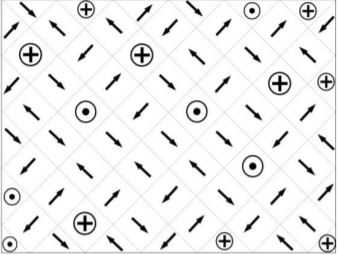
\includegraphics[width=.45\linewidth]{Домены1.png}
				\caption{Ориентация магнитных моментов доменов в ферромагнетике}
				\label{fig:3}
			\end{figure}
			Кусок ферромагнетика разделяется на области - домены, в которых намагниченность преимущественно направленна вдоль одной из кристаллографических осей
		\end{center}
	\end{frame}
	
	\begin{frame}
		\frametitle{Теория}
		\framesubtitle{Формирование доменов}
		\begin{center}
			\begin{figure}[h!]
				\centering
				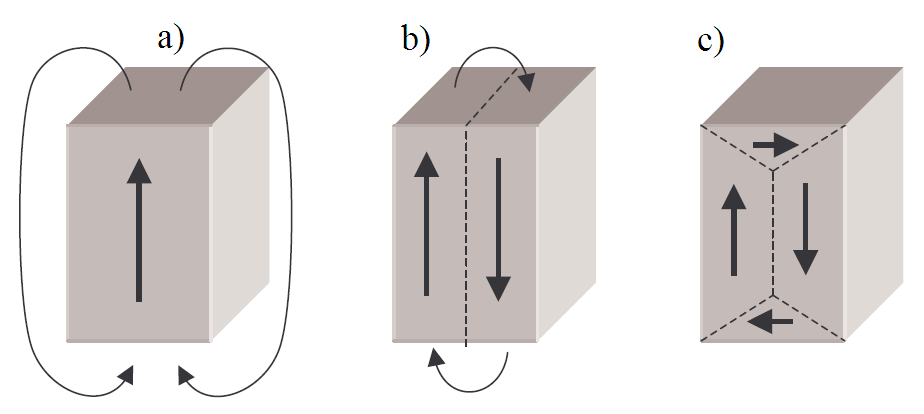
\includegraphics[width=.7\linewidth]{Домены2.png}
				\caption{Разделение ферромагнитного материала на магнитные домены снижает магнитостатическую энергию}
				\label{fig:3}
			\end{figure}
		Большая область из ферромагнитного материала создаст большое магнитное поле, которое требует большого количества энергии, поэтому большие области разделяются на малые домены.
		\end{center}
	\end{frame}

	\begin{frame}
		\frametitle{Теория}
		\framesubtitle{Формирование доменов}
		\begin{center}
			\begin{figure}[h!]
				\centering
				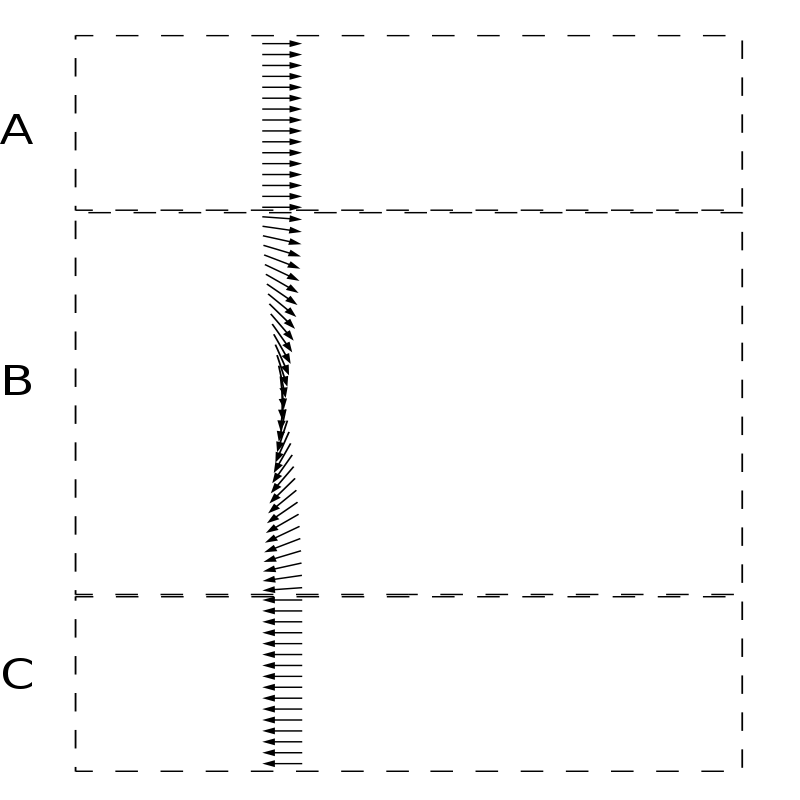
\includegraphics[width=.35\linewidth]{Домены4.png}
				\caption{A и C - Домены с противоположной намагниченстью, B - доменная стенка}
				\label{fig:3}
			\end{figure}
			Каждый раз, когда область намагниченности разделяется на два домена, это создает доменную стенку между доменами, где противоположные магнитные моменты соседствуют. Обменное взаимодействие которая создает намагниченность - это сила, которая стремится выровнять близлежащие диполи так, чтобы они указывали в одном направлении. Чтобы заставить соседние диполи указывать в разных направлениях, требуется энергия.
		\end{center}
	\end{frame}
	
	\begin{frame}
		\frametitle{Теория}
		\framesubtitle{Формирование домена}
		\begin{center}
			\begin{figure}[h!]
				\centering
				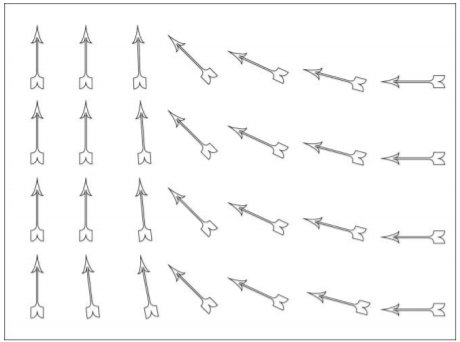
\includegraphics[width=.5\linewidth]{Домены3.png}
				\caption{Переходная область домена к доменной стенке}
				\label{fig:3}
			\end{figure}
			Таким образом, чистое количество энергии, которое уменьшается при разделении домена, равно разнице между сохраненной энергией магнитного поля и дополнительной энергией, необходимой для создания доменной стенки.
		\end{center}
	\end{frame}
	
	\begin{frame}
		\frametitle{Теория}
		\framesubtitle{Процесс намагничивания}
		\begin{center}
			\begin{figure}[h!]
				\centering
				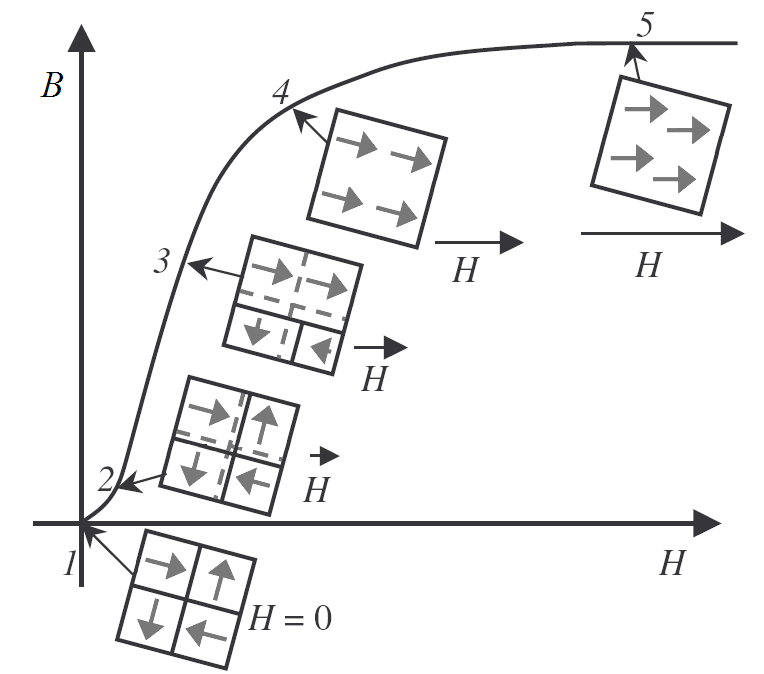
\includegraphics[width=.4\linewidth]{Домены5.png}
				\caption{Изменение доменов в зависимости от приложенного поля}
				\label{fig:3}
			\end{figure}
		\begin{itemize}
			\item Расширение границ доменов, намагниченность которых совпадает с направлением поля (1-3)
			\item Вращение магнитного момента остальных доменов в направлении поля (3-4)
			\item Переориентация спинов спонтанно намагниченных областей, вызванных тепловым движением.
		\end{itemize}
		\end{center}
	\end{frame}

	\begin{frame}
		\frametitle{Теория} 
		\framesubtitle{Индуктивность катушки}
		\begin{center}
				Вычислить индуктивность катушки можно, собрав данную схему и записав отношение напряжений на блоке питания и резисторе : 
				\begin{figure}[h!]
					\centering
					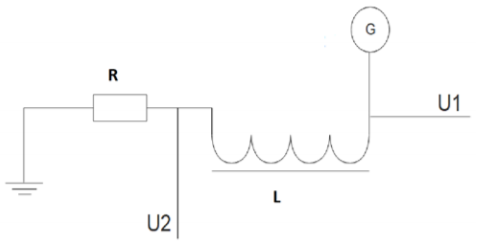
\includegraphics[width=.5\linewidth]{схема1.png}
					\caption{Цепь для определения индуктивности}
					\label{fig:1}
				\end{figure}
				\begin{equation}
				\frac{U_1}{U_2} = \sqrt{1 + (\frac{\omega L}{R})^2}
				\end{equation}
				То есть:
				\begin{equation}
					L = \frac{R}{2 \pi \nu}\sqrt{(\frac{U_1}{U_2})^2 - 1}
				\end{equation}
		\end{center}
	\end{frame}

	\begin{frame}
		\frametitle{Теория} 
		\framesubtitle{Магнитная восприимчивость сердечника}
		\begin{center}
			Чтобы найти магнитную восприимчивость сердечника запишем закон Фарадея и 4 уравнение Максвелла:
			\begin{equation}
			\begin{gathered}
			\EDS = -\frac{d\Phi}{dt}\\
			\oint\limits\mathbf{H}\cdot d\mathbf{l} = I
			\end{gathered}
			\end{equation}
			Отсюда получим:
			\begin{equation}
			\begin{gathered}
			L I = S N \mu \mu_0 H\\
			H = \frac{N I}{2 \pi} \ln{\frac{R}{r}}
			\end{gathered}
			\end{equation}
			То есть:
			\begin{equation}
			\mu = \frac{2 \pi L}{ \mu_0 N^2 h \ln{\frac{R}{r}}}
			\end{equation}
		\end{center}
	\end{frame}
	
	\begin{frame}
		\frametitle{Теория} 
		\framesubtitle{Гистерезис}
		\begin{center}
			\begin{itemize}
			\item Для исследования магнитного гистерезиса можно использовать две схемы:
			\begin{figure}[ht]
				\begin{minipage}{.45\textwidth}
					\label{figure1}
					\centering
					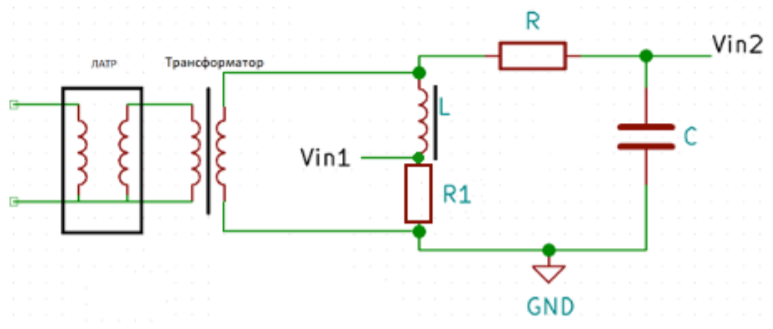
\includegraphics[width=1.0\linewidth]{схема2.png}
					\caption{Схема с 1 катушкой}
				\end{minipage}
				\begin{minipage}{.45\textwidth}
					\label{figure2}
					\centering
					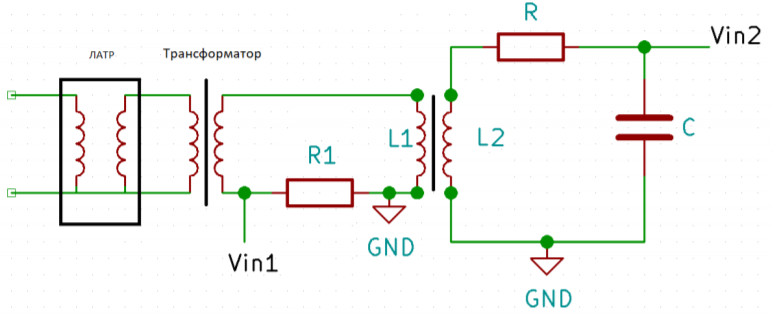
\includegraphics[width=1.0\linewidth]{схема3.png}
					\caption{Схема с 2 катушками}	
				\end{minipage}
			\label{fig:2}
			\end{figure}
			\item Используя 4 уравнение Максвелла и закон Фарадея получим:
			\begin{equation}
				\begin{gathered}
				H = \frac{N_1 I}{\pi D} \\
				V = -\frac{d\Phi}{dt} = -S N_i\frac{dB}{dt} \\
				\end{gathered}
			\end{equation}
			\end{itemize}
		\end{center}
	\end{frame}

\begin{frame}
	\frametitle{Теория}
	\framesubtitle{Гистерезис} 
	\begin{center}
		Запишем напряжение на конденсаторе:
		\begin{equation}
			V_c \approx \frac{1}{RC}\int V dt = S N_i B
		\end{equation}	
		Отсюда:
		\begin{equation}
			\begin{gathered}
			H = \frac{N_1 I}{\pi D} \\
			B = V_2 R C \frac{1}{R C}
			\end{gathered}
		\end{equation}
		Кроме того, нам понадобятся связь намагниченности $M$ и полей $B$ и $H$, а также магнитная проницаемость $\chi$:
		\begin{equation}
		\begin{gathered}
		\mathbf{B} =\mu_0(\mathbf{H} + \textbf{M})\\
		\chi = \frac{dM}{dH}
		\end{gathered}
		\end{equation}
	\end{center}
\end{frame}

	\begin{frame}
		\frametitle{Оборудование} 
		\begin{center}
			\begin{itemize}
				\item Цифровой осциллограф Rigol
				\item ЛАТР
				\item Понижающий трансформатор
				\item Клемник для сборки электрических цепей
				\item Толстая медная проволока
				\item Тонкая медная проволока
				\item Ферритовый сердечник
				\item Резистор сопротивлением 100 мОм
				\item Резистор сопротивлением 95 Ом
				\item Резистор сопротивлением 795 кОм
				\item Конденсатор ёмкостью 1 мкФ
			\end{itemize}
		\end{center}
	\end{frame}

	\begin{frame}
		\frametitle{Определение индуктивности катушки} 
		\begin{center}
			\begin{figure}[h!]
				\centering
				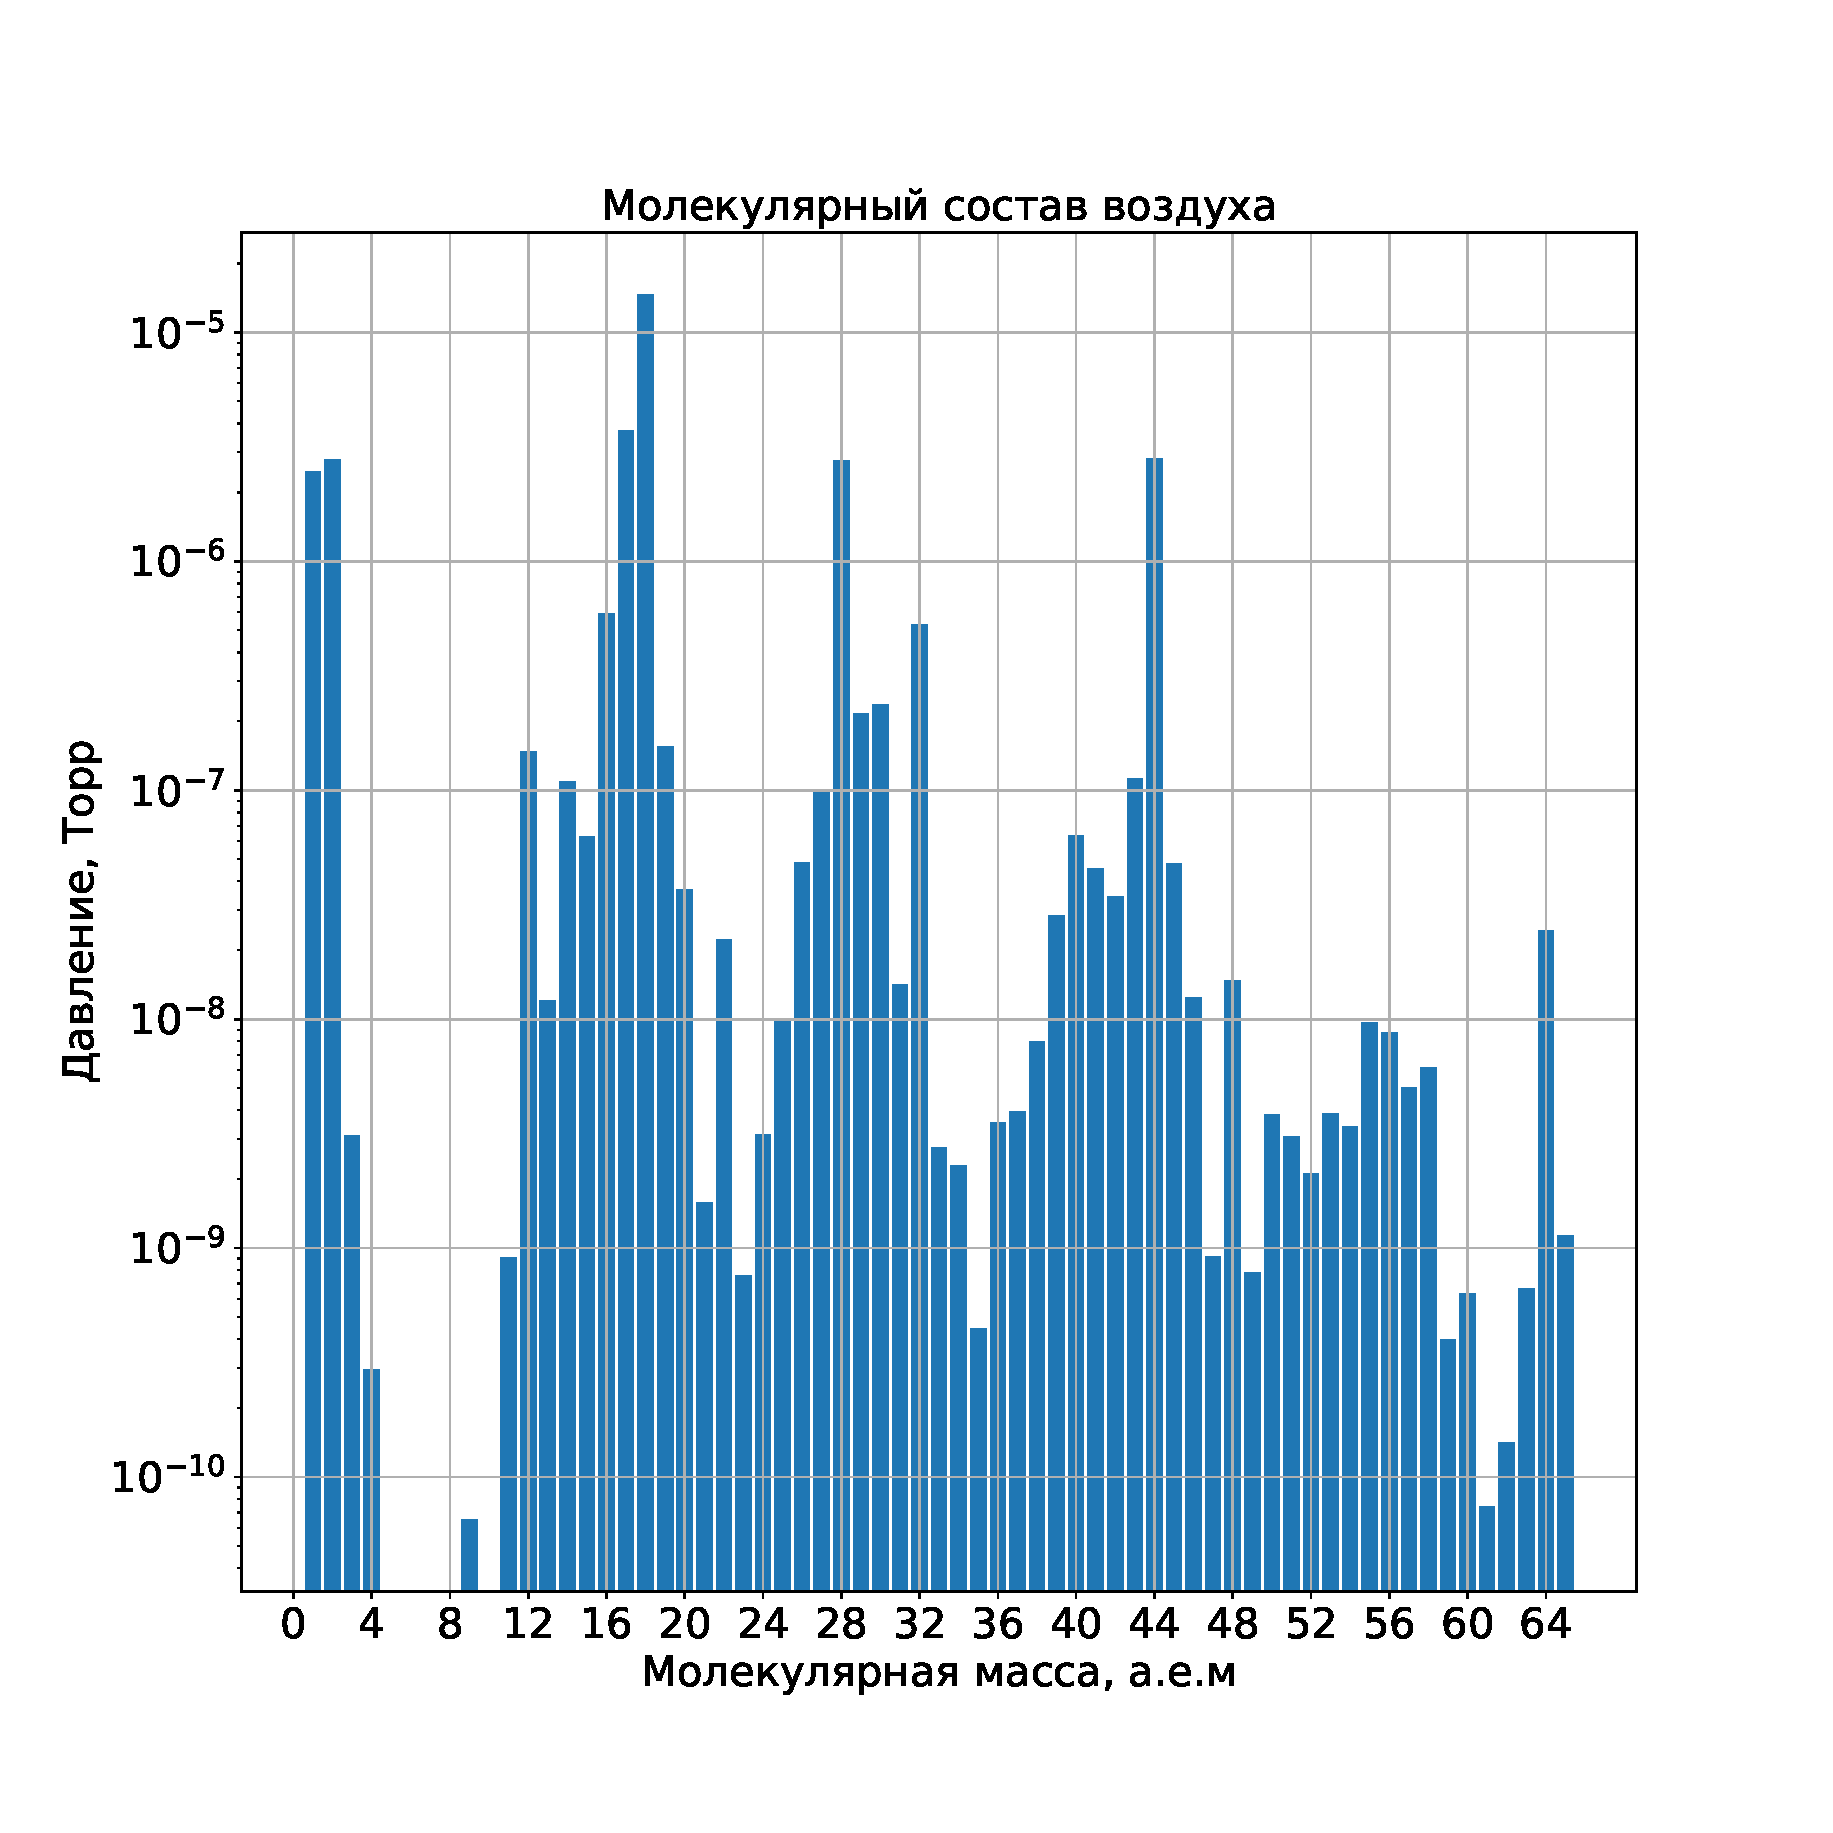
\includegraphics[width=.5\linewidth]{Lab2_1.eps}
				\caption{На графике изображены две прямые: прямая, построенная по экспериментальным данным с помощью МНК и прямая, построенная с помощью взвешенного МНК}
				\label{fig:3}
			\end{figure}
		\end{center}
	\end{frame}

	\begin{frame}
		\frametitle{Вычисление проницаемости} 
		\begin{center}
			За основу был взят график, построенный по взвешенному МНК, так как при предыдущих измерениях индуктивности катушки получившийся результат лучше соотносился с заявленной индуктивностью и показателями точных приборов.
			\newline
			Получившаяся индуктивность с учетом погрешностей:
			\begin{equation}	
			L = 2.73 \pm 0.10\text{мГн}
			\end{equation}
			С помощью вычисленной индуктивности можно найти магнитную проницаемость:
			\begin{equation}
			\mu = 2.08 \pm 0.08\frac{\text{Гн}}{\text{м}}
			\end{equation}
		\end{center}
	\end{frame}

	\begin{frame}
		\frametitle{Гистерезис}
		 \framesubtitle{Схема с 1 катушкой}
		\begin{center}
			\begin{figure}[h!]
				\centering
				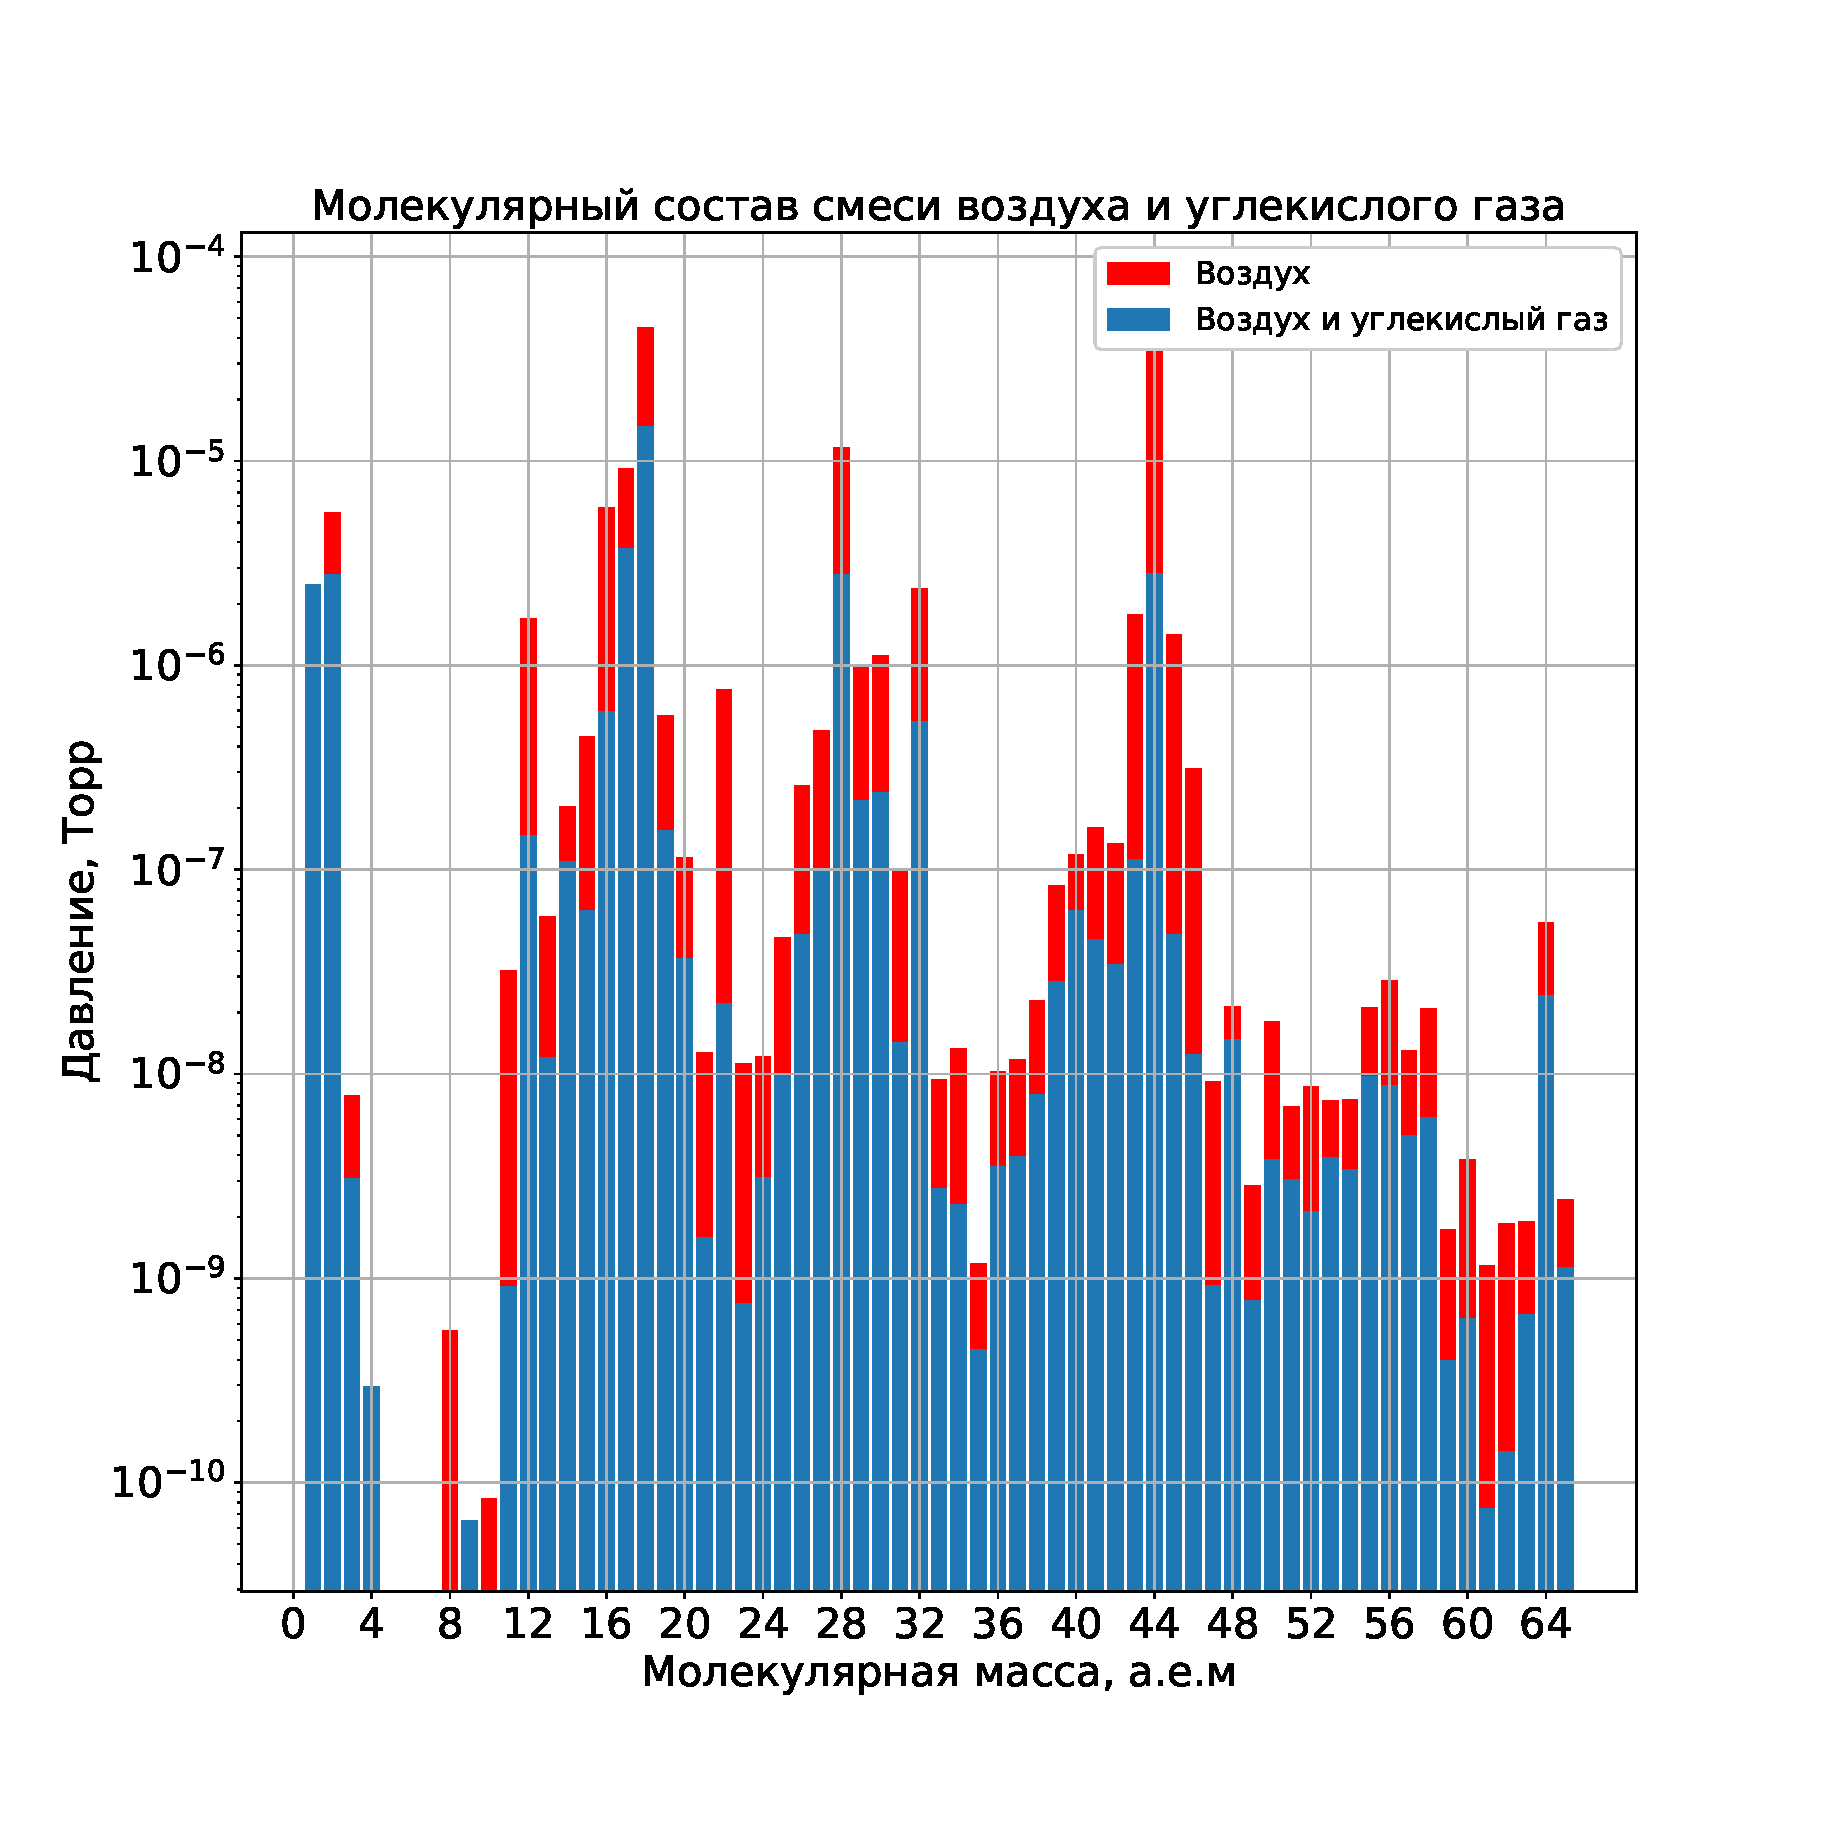
\includegraphics[width=.45\linewidth]{Lab2_2.eps}
				\caption{Петля гистерезиса для ферритового сердечника. Схема 1}
				\label{fig:3}
			\end{figure}
		Графики довольно сильно искажались уже при очень малых напряжениях, поэтому было решено собрать данные используя схему с двумя катушками
		\end{center}
	\end{frame}

	\begin{frame}
		\frametitle{Гистерезис}
		\framesubtitle{Схема с 2 катушками}
		\begin{center}
			\begin{figure}[h!]
				\centering
				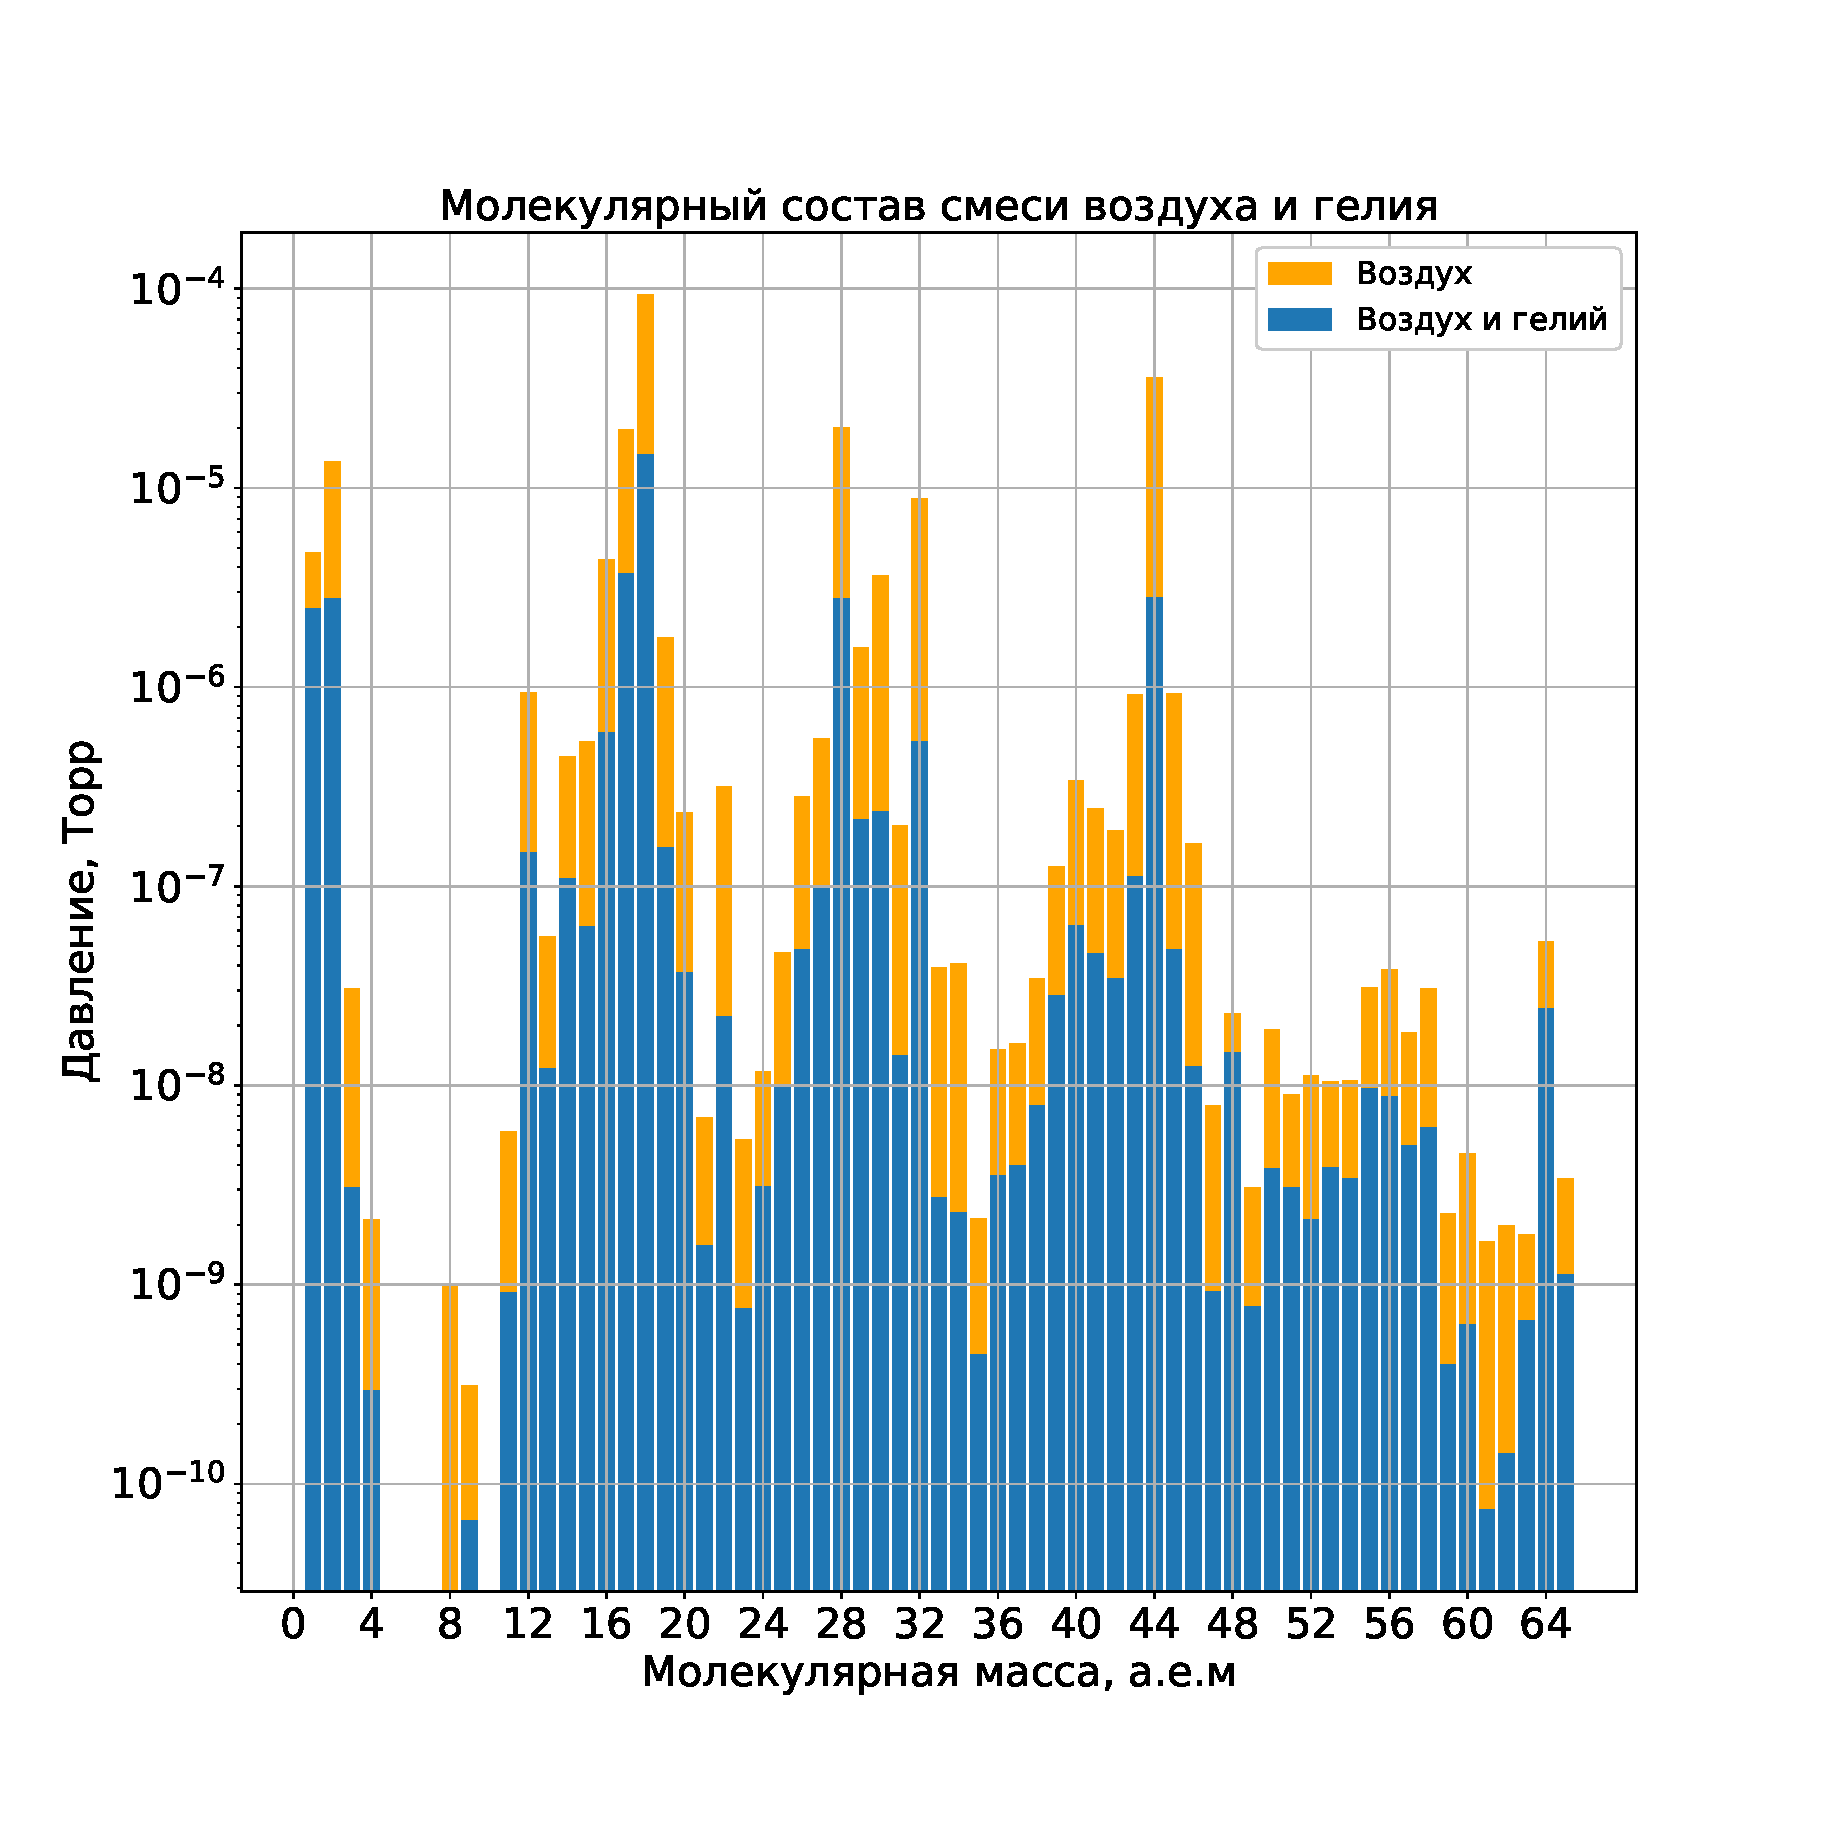
\includegraphics[width=.65\linewidth]{Lab2_3.eps}
				\caption{Собранные с осциллографа данные}
				\label{fig:3}
			\end{figure}
		\end{center}
	\end{frame}
	
	\begin{frame}
		\frametitle{Гистерезис}
		\framesubtitle{Намагниченность}
		\begin{center}
			\begin{figure}[h!]
				\centering
				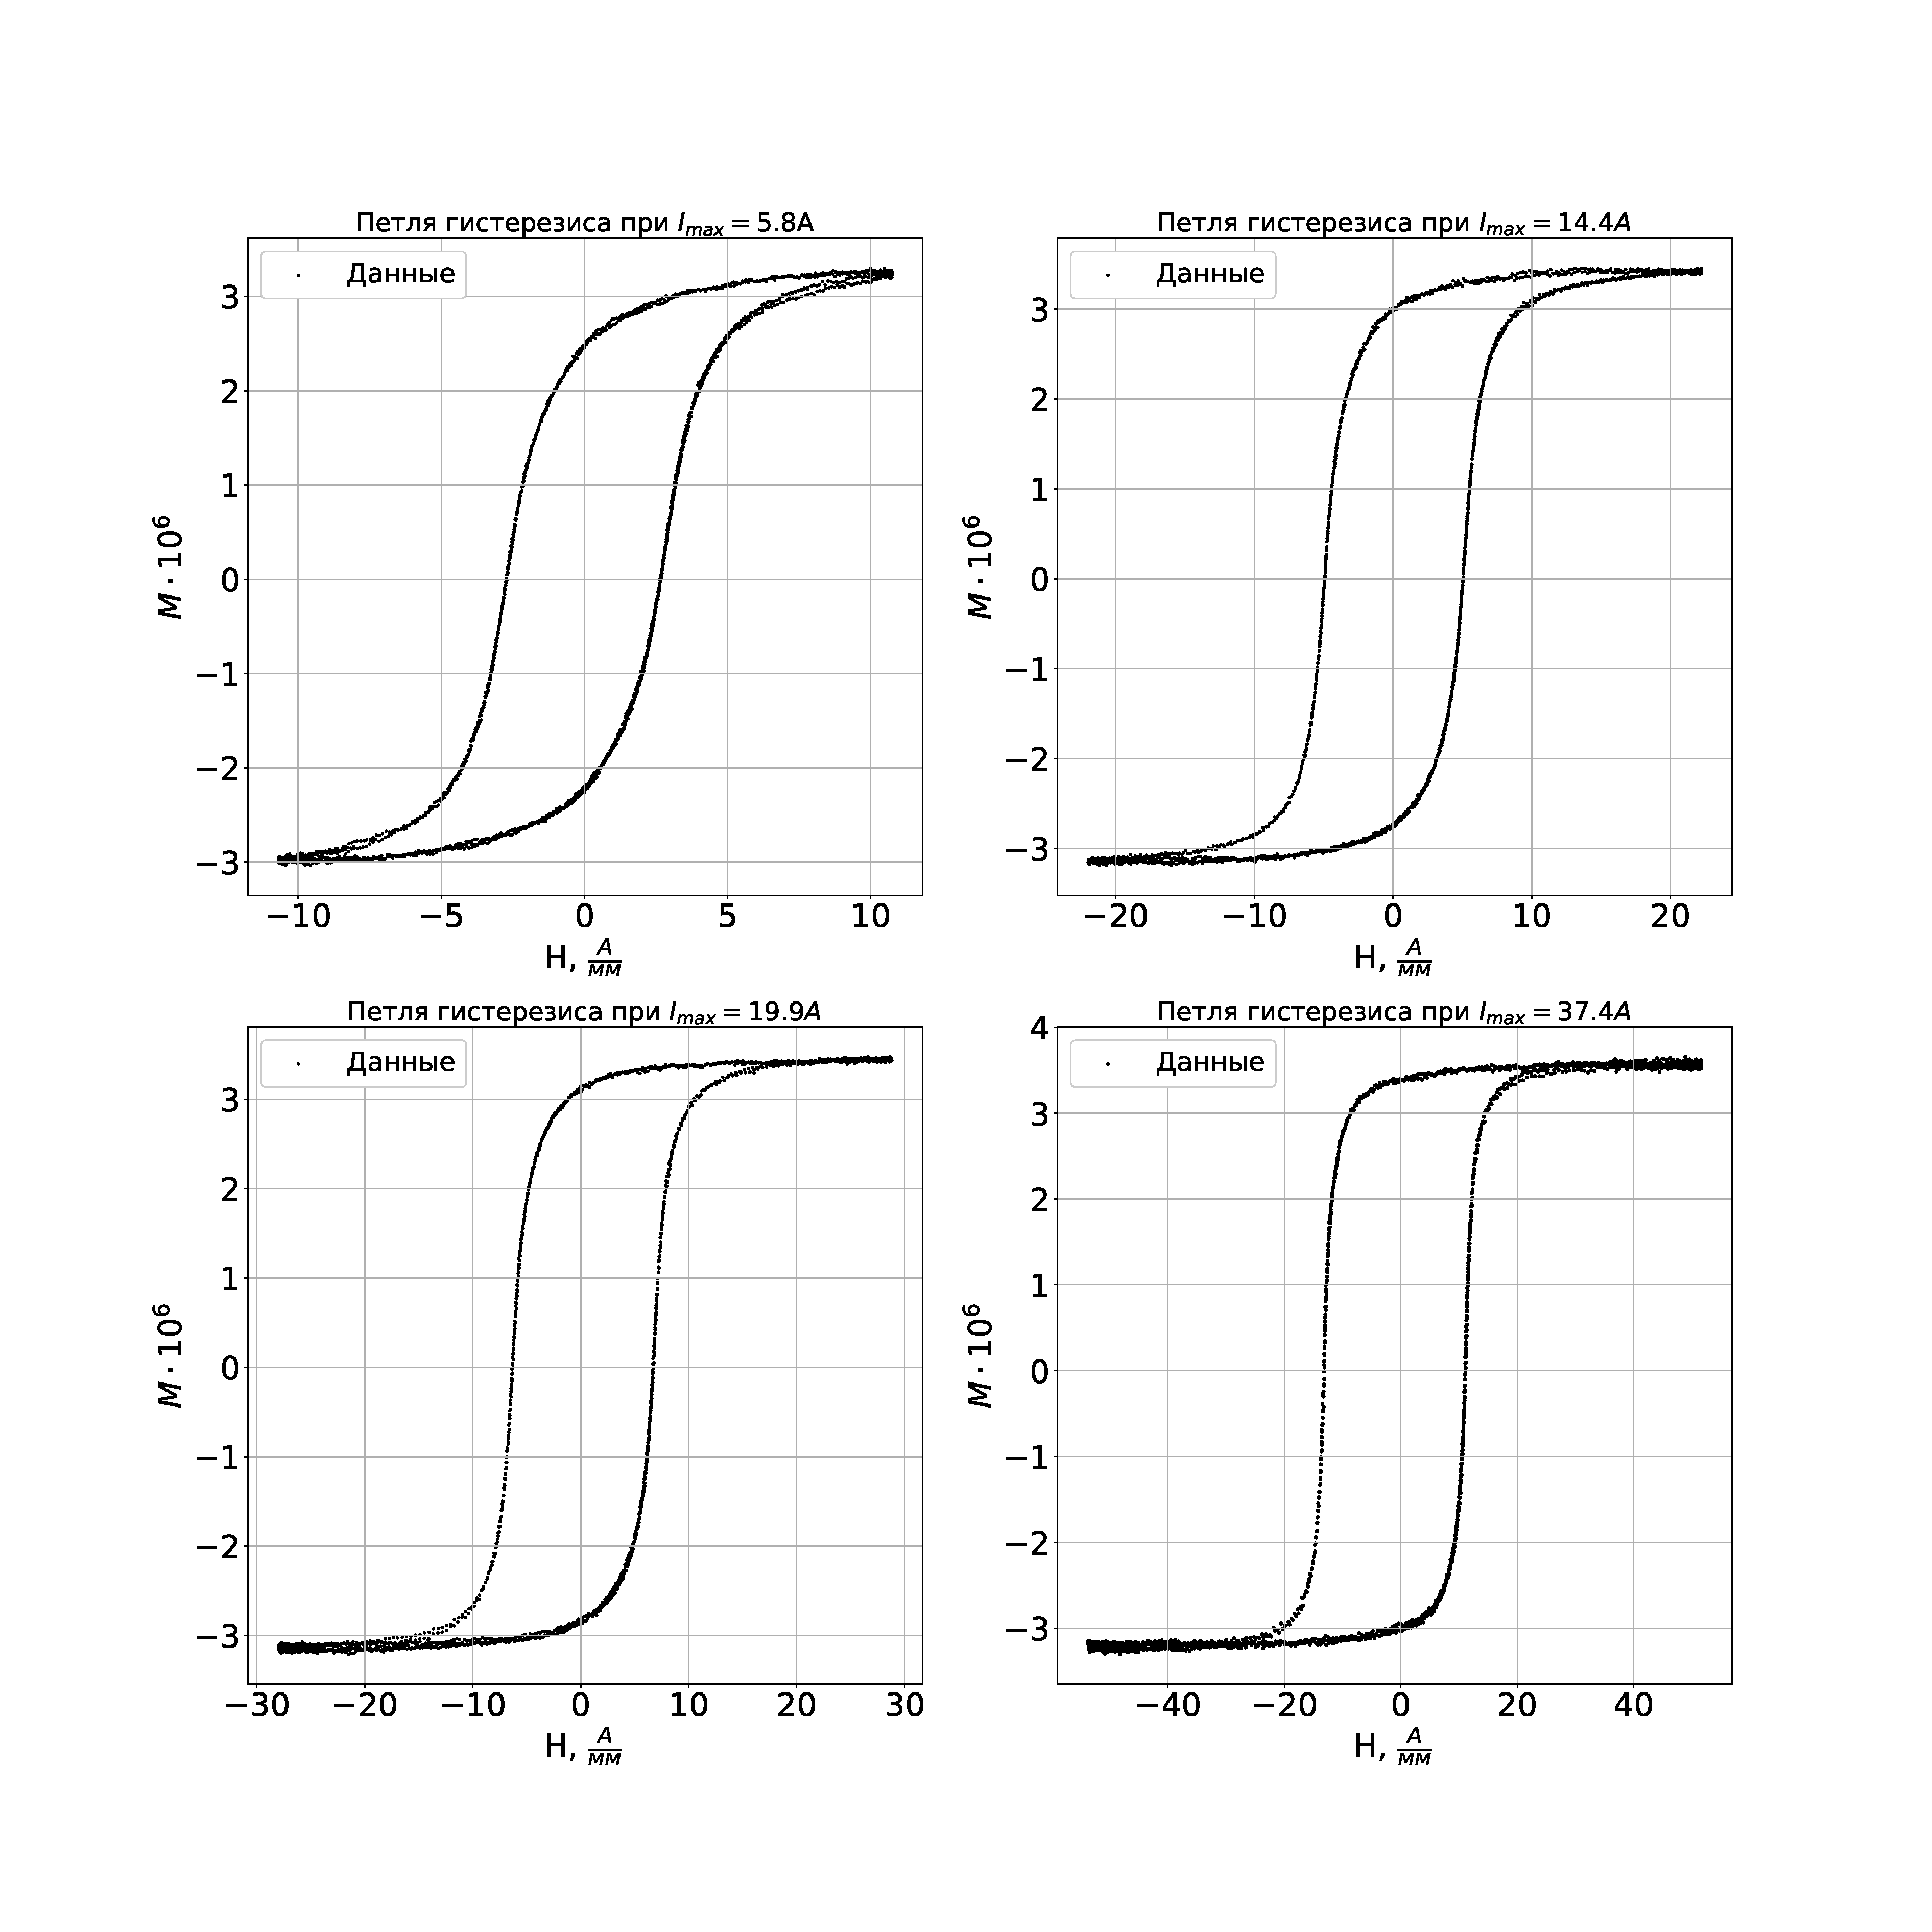
\includegraphics[width=.65\linewidth]{lab2_4.eps}
				\caption{Собранные с осциллографа данные}
				\label{fig:3}
			\end{figure}
		\end{center}
	\end{frame}
	
	\begin{frame}
		\frametitle{Гистерезис}
		\framesubtitle{Магнитная восприимчивость}
		\begin{center}
			\begin{figure}[h!]
				\centering
				\includegraphics[width=.65\linewidth]{Lab2_5.png}
				\caption{Собранные с осциллографа данные}
				\label{fig:3}
			\end{figure}
		\end{center}
	\end{frame}

	\begin{frame}
		\frametitle{Гистерезис}
		\framesubtitle{Магнитная восприимчивость}
		\begin{center}
			\begin{figure}[h!]
				\centering
				\includegraphics[width=.5\linewidth]{Lab2_14.eps}
				\caption{Линеаризация участка петли для поиска максимальной восприимчивости при $I_{max} = 5.8$А}
				\label{fig:3}
			\end{figure}
		\end{center}
	\end{frame}

	\begin{frame}
		\frametitle{Гистерезис}
		\framesubtitle{Магнитная восприимчивость}
		\begin{center}
			\begin{figure}[h!]
				\centering
				\includegraphics[width=.45\linewidth]{Lab2_15.eps}
				\caption{График зависимости восприимчивости от поля при $I_{max} = 5.8$А}
				\label{fig:3}
			\end{figure}
		\begin{equation}
			\chi_{max} \approx 2.3 \cdot 10^3
		\end{equation}
		\end{center}
	\end{frame}
	
	\begin{frame}
		\frametitle{Гистерезис}
		\framesubtitle{Магнитная восприимчивость}
		\begin{center}
			\begin{figure}[h!]
				\centering
				\includegraphics[width=.5\linewidth]{Lab2_11.eps}
				\caption{Линеаризация участка петли для поиска максимальной восприимчивости при $I_{max} = 14.4$А}
				\label{fig:3}
			\end{figure}
		\end{center}
	\end{frame}
	
	\begin{frame}
		\frametitle{Гистерезис}
		\framesubtitle{Магнитная восприимчивость}
		\begin{center}
			\begin{figure}[h!]
				\centering
				\includegraphics[width=.45\linewidth]{Lab2_10.eps}
				\caption{График зависимости восприимчивости от поля при $I_{max} = 14.4$А}
				\label{fig:3}
			\end{figure}
			\begin{equation}
			\chi_{max} \approx 2.42 \cdot 10^3
			\end{equation}
		\end{center}
	\end{frame}

	\begin{frame}
		\frametitle{Гистерезис}
		\framesubtitle{Магнитная восприимчивость}
		\begin{center}
			\begin{figure}[h!]
				\centering
				\includegraphics[width=.5\linewidth]{Lab2_8.eps}
				\caption{Линеаризация участка петли для поиска максимальной восприимчивости при $I_{max} = 19.9$А}
				\label{fig:3}
			\end{figure}
		\end{center}
	\end{frame}
	
	\begin{frame}
		\frametitle{Гистерезис}
		\framesubtitle{Магнитная восприимчивость}
		\begin{center}
			\begin{figure}[h!]
				\centering
				\includegraphics[width=.45\linewidth]{Lab2_9.eps}
				\caption{График зависимости восприимчивости от поля $I_{max} = 19.9$А}
				\label{fig:3}
			\end{figure}
			\begin{equation}
			\chi_{max} \approx 2.45 \cdot 10^3
			\end{equation}
		\end{center}
	\end{frame}

	\begin{frame}
		\frametitle{Гистерезис}
		\framesubtitle{Магнитная восприимчивость}
		\begin{center}
			\begin{figure}[h!]
				\centering
				\includegraphics[width=.5\linewidth]{Lab2_13.eps}
				\caption{Линеаризация участка петли для поиска максимальной восприимчивости $I_{max} = 37.4$А}
				\label{fig:3}
			\end{figure}
		\end{center}
	\end{frame}
	
	\begin{frame}
		\frametitle{Гистерезис}
		\framesubtitle{Магнитная восприимчивость}
		\begin{center}
			\begin{figure}[h!]
				\centering
				\includegraphics[width=.45\linewidth]{Lab2_12.eps}
				\caption{График зависимости восприимчивости от поля $I_{max} = 37.4$А}
				\label{fig:3}
			\end{figure}
			\begin{equation}
			\chi_{max} \approx 2.51 \cdot 10^3
			\end{equation}
		\end{center}
	\end{frame}

	\begin{frame}
		\frametitle{Гистерезис}
		\framesubtitle{Коэрцитивная сила}
		\begin{center}
			\begin{figure}[h!]
				\centering
				\includegraphics[width=.45\linewidth]{Lab2_6.eps}
				\caption{График зависимости коэрцитивной силы от максимальной силы тока в цепи}
				\label{fig:3}
			\end{figure}
		По получившемуся результату можно предположить, что коэрцитивная сила ведет себя линейно по отношению к току
		\end{center}
	\end{frame}

	\begin{frame}
		\frametitle{Гистерезис}
		\framesubtitle{Остаточная намагниченность}
		\begin{center}
			\begin{figure}[h!]
				\centering
				\includegraphics[width=.4\linewidth]{Lab2_7.eps}
				\caption{График зависимости остаточной намагниченности от максимальной силы тока в цепи}
				\label{fig:3}
			\end{figure}
		Последняя точка на графике выше не учитывается из-за того, что остаточная намагниченность при большом токе соответствует насыщению.
		\end{center}
	\end{frame}

	\begin{frame}
		\frametitle{Гистерезис}
		\framesubtitle{Коэрцитивная сила и намагниченность}
		\begin{center}
			\begin{equation}
			\begin{gathered}
			\text{При } I = 5.77 \text{А}:
			\begin{gathered}
			H_c\approx 2.68 \; \frac{\text{А}}{\text{мм}}\\
			B_r\approx 4.05 \; \text{Тл}
			\end{gathered}\\ \\
			\text{При } I = 14.38 \text{А}:
			\begin{gathered}
			H_c\approx 4.99 \; \frac{\text{А}}{\text{мм}}\\
			B_r\approx 4.91 \; \text{Тл}
			\end{gathered}\\ \\
			\text{При } I = 19.87 \text{А}:
			\begin{gathered}
			H_c\approx 6.51 \; \frac{\text{А}}{\text{мм}}\\
			B_r\approx 5.11 \; \text{Тл}
			\end{gathered}\\ \\
			\text{При } I = 37.36 \text{А}:
			\begin{gathered}
			H_c\approx 12.07 \; \frac{\text{А}}{\text{мм}}\\
			B_r\approx 5.41 \; \text{ Тл}
			\end{gathered}\\ \\
			\end{gathered}
				\end{equation}
		\end{center}
	\end{frame}

\end{document}